\begin{figure}[htbp]
    \centering
    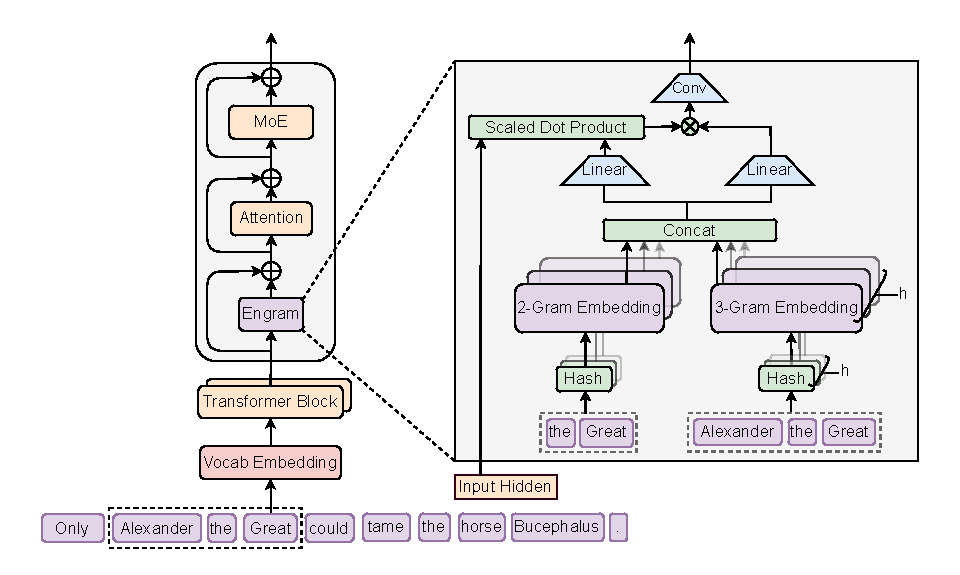
\includegraphics[width=0.95\linewidth]{figs/engram_arch.pdf}
    \caption{
        \textbf{The Engram Architecture.} The module augments the backbone by retrieving static $N$-gram memory and fusing it with dynamic hidden states via context-aware gating. This module is applied only to specific layers to decouple memory from compute, leaving the standard input embedding and un-embedding module intact.
    }
    \label{fig:dse_architecture}
\end{figure}


\section{Architecture}
\label{sec:architecture}

\subsection{Overview}
\label{sec:arch_overview}

As shown in \autoref{fig:dse_architecture}, Engram is a conditional memory module designed to augment the Transformer backbone by structurally separating static pattern storage from dynamic computation. Formally, given an input sequence $X = (x_1, \dots, x_T)$ and hidden states $\mathbf{H}^{(\ell)} \in \mathbb{R}^{T \times d}$ at layer $\ell$, the module processes each position $t$ in two functional phases: \textbf{retrieval and fusion}. 
First, as detailed in \autoref{sec:engram_retrieval}, we extract and compress suffix $N$-grams to deterministically retrieve static embedding vectors via hashing.
Subsequently, in \autoref{sec:engram_fusion}, these retrieved embeddings are dynamically modulated by the current hidden state and refined via a lightweight convolution.
Finally, we discuss the integration with multi-branch architectures in \autoref{sec:engram_hc_integration} and the system-level design in \autoref{sec:system_efficiency}.



\subsection{Sparse Retrieval via Hashed $N$-grams}
\label{sec:engram_retrieval}
The first phase maps local contexts to static memory entries, involving tokenizer compression and retrieving embeddings via deterministic hashing. 


\paragraph{Tokenizer Compression}
While $N$-gram models typically operate directly on tokenizer outputs, standard subword tokenizers prioritize \textit{lossless reconstruction}, often assigning disjoint IDs to semantically equivalent terms~(e.g., \texttt{Apple} vs. \texttt{\textvisiblespace apple})~\citep{kudo2018sentencepiecesimplelanguageindependent,li2023starcodersourceyou}. To maximize semantic density, we implement a vocabulary projection layer. Specifically, we pre-compute a surjective function $\mathcal{P}: V \to V'$ that collapses raw token IDs into canonical identifiers based on normalized textual equivalence (using NFKC~\citep{UAX15-NFKC}, lowercasing, etc.). In practice, this process achieves a 23\% reduction in the effective vocabulary size for a 128k tokenizer (see ~\autoref{appendix:token_compression}). 
Formally, for a token at position $t$, we map its raw ID $x_t$ to a canonical ID $x'_t = \mathcal{P}(x_t)$ to form the suffix $N$-gram $g_{t,n} = (x'_{t-n+1}, \dots, x'_t)$.




\paragraph{Multi-Head Hashing.}

Directly parameterizing the combinatorial space of all possible $N$-grams is intractable. Following \citet{tito2017hash}, we adopt a hashing-based approach. To mitigate collisions, we employ $K$ distinct hash heads for each $N$-gram order $n$. Each head $k$ maps the compressed context to an index within an embedding table $\mathbf{E}_{n,k}$ (of prime size $M_{n,k}$) via a deterministic function $\phi_{n,k}$:
\begin{equation}
    z_{t,n,k} \triangleq \phi_{n,k}(g_{t,n}), \quad
    \mathbf{e}_{t,n,k} = \mathbf{E}_{n,k}[z_{t,n,k}].
\end{equation}
In practice, $\phi_{n,k}$ is implemented as a lightweight multiplicative-XOR hash. We construct the final memory vector $\mathbf{e}_t \in \mathbb{R}^{d_{\text{mem}}}$ by concatenating all retrieved embeddings:
\begin{equation}
    \mathbf{e}_t \triangleq \mathop{\Vert}_{n=2}^{N} \mathop{\Vert}_{k=1}^{K} \mathbf{e}_{t,n,k}.
\end{equation}




\subsection{Context-aware Gating}
\label{sec:engram_fusion}
The retrieved embeddings $\mathbf{e}_t$ serve as context-independent priors. Being static, however, they inherently lack contextual adaptability and may suffer from noise due to hash collisions or polysemy~\citep{haber-poesio-2024-polysemy}.
To enhance expressivity and resolve this ambiguity, we employ a context-aware gating mechanism inspired by Attention~\citep{vaswani2017attention,bahdanau2014neural}. Specifically, we utilize the current hidden state $\mathbf{h}_t$—which has aggregated global context via preceding attention layers—as a dynamic Query, while the retrieved memory $\mathbf{e}_t$ serves as the source for both Key and Value projections:
\begin{equation}
    \mathbf{k}_t = \mathbf{W}_K \mathbf{e}_t, \quad \mathbf{v}_t = \mathbf{W}_V \mathbf{e}_t
\end{equation}
where $\mathbf{W}_K, \mathbf{W}_V$ are learnable projection matrices. To ensure gradient stability~\citep{pmlr-v202-dehghani23a}, we apply RMSNorm~\citep{zhang2019root} to the Query and Key before computing the scalar gate $\alpha_t \in (0, 1)$: 
\begin{equation}
    \alpha_t = \sigma\left( \frac{\text{RMSNorm}(\mathbf{h}_t)^\top  \text{RMSNorm}(\mathbf{k}_t)}{\sqrt{d}} \right).
\end{equation}
The gated output is defined as $\tilde{\mathbf{v}}_t = \alpha_t \cdot \mathbf{v}_t$. This design enforces semantic alignment: if the retrieved memory $\mathbf{e}_t$ contradicts the current context $\mathbf{h}_t$, the gate $\alpha_t$ tends toward zero, effectively suppressing the noise.

Finally, to expand the receptive field and enhance the model's non-linearity, we introduce a short, depthwise causal convolution~\citep{gu2021efficiently,peng2023rwkv}. Let $\tilde{\mathbf{V}} \in \mathbb{R}^{T \times d}$ denote the sequence of gated values. Using a kernel size $w$ (set to 4), dilation $\delta$ (set to the max $N$-gram order) and SiLU activation~\citep{elfwing2018sigmoid}, the final output $\mathbf{Y}$ is computed as: 
\begin{equation}
    \mathbf{Y} = \text{SiLU}\left( \text{Conv1D}( \text{RMSNorm}(\tilde{\mathbf{V}}) ) \right) + \tilde{\mathbf{V}}, 
\end{equation}
The Engram module is integrated into the backbone via a residual connection: $\mathbf{H}^{(\ell)} \leftarrow \mathbf{H}^{(\ell)} + \mathbf{Y}$, followed by the standard Attention and MoE. 
Crucially, Engram is not applied to every layer; its specific placement is optimized to balance modeling effectiveness against the system-level latency constraints detailed in \autoref{sec:system_efficiency}.


\begin{figure}[!t]
    \centering
    \includegraphics[width=0.95\linewidth]{figs/engram_system.pdf}
    \caption{
    \textbf{System implementation of Engram.} 
    (a) Training Phase: The massive embedding tables are sharded across available GPUs. An All-to-All communication primitive is employed to retrieve active embedding rows across devices. 
    (b) Inference Phase: Engram tables are offloaded to host memory. By exploiting the deterministic retrieval logic, the host asynchronously prefetches and transfers embeddings, overlapping communication with the on-device computation of preceding Transformer blocks.
    }
    \label{fig:engram_system}
\end{figure}

\subsection{Integration with Multi-branch Architecture}
\label{sec:engram_hc_integration}

In this work, rather than standard single-stream connections~\citep{he2016deep}, we adopt the advanced multi-branch architecture as our default backbone, chosen for its superior modeling capabilities~\citep{larsson2016fractalnet,zhu2025hyperconnections,xie2025mhcmanifoldconstrainedhyperconnections,szegedy2015going}. A defining characteristic of this architecture is the expansion of the residual stream into $M$ parallel branches, where information flow is modulated by learnable connection weights.

Although the Engram module is inherently topology-agnostic, adapting it to this multi-branch framework necessitates structural optimization to balance efficiency and expressivity. 
Specifically, we implement a parameter-sharing strategy: a single sparse embedding table and a Value projection matrix $\mathbf{W}_V$ are shared across all $M$ branches, whereas $M$ distinct Key projection matrices $\{\mathbf{W}_K^{(m)}\}_{m=1}^M$ are employed to enable branch-specific gating behaviors.
For the $m$-th branch with hidden state $\mathbf{h}_t^{(m)}$, the branch-specific gating signal is computed as:
\begin{equation}
    \alpha_t^{(m)} = \sigma\left( \frac{\text{RMSNorm}(\mathbf{h}_t^{(m)})^\top \text{RMSNorm}(\mathbf{W}_K^{(m)} \mathbf{e}_t)}{\sqrt{d}} \right).
\end{equation}
The retrieved memory is then modulated by these independent gates applied to the shared value vector: $\mathbf{u}_t^{(m)} = \alpha_t^{(m)} \cdot (\mathbf{W}_V \mathbf{e}_t)$. This design allows the linear projections (one $\mathbf{W}_V$ and $M$ distinct $\mathbf{W}_K^{(m)}$) to be fused into a single dense FP8 matrix multiplication, maximizing the compute utilization of modern GPUs. Unless otherwise stated, all experiments utilize this integration with Manifold-Constrained Hyper-Connections~($M=4$)~\citep{xie2025mhcmanifoldconstrainedhyperconnections}.

\subsection{System Efficiency: Decoupling Compute and Memory}
\label{sec:system_efficiency}

Scaling model parameters is often constrained by the limited capacity of GPU high-bandwidth memory (HBM). However, unlike MoE which relies on runtime hidden states for dynamic routing, Engram employs a deterministic retrieval mechanism based solely on input token IDs, naturally decoupling parameter storage from computation. This predictability facilitates specialized optimization strategies for both training and inference, as illustrated in \autoref{fig:engram_system}.

During training, to accommodate large-scale embedding tables, we employ standard model parallelism by sharding the tables across available GPUs. An All-to-All communication primitive is used to gather active rows in the forward pass and dispatch gradients in the backward pass, enabling the total memory capacity to scale linearly with the number of accelerators.

During inference, this deterministic nature enables a prefetch-and-overlap strategy. Since memory indices are known prior to the forward pass, the system can asynchronously retrieve embeddings from abundant host memory via PCIe. To effectively mask communication latency, the Engram module is placed at specific layers within the backbone, leveraging the computation of preceding layers as a buffer to prevent GPU stalls.
This necessitates a hardware-algorithm co-design strategy: while placing Engram deeper extends the compute window available for hiding latency, our ablation in \autoref{sec:ablation_structural} shows that modeling performance favors early intervention to offload local pattern reconstruction. Therefore, the optimal placement must simultaneously satisfy both modeling and system latency constraints.


Furthermore, natural language $N$-grams inherently follow a Zipfian distribution~\citep{piantadosi2014zipf,Chao1950HumanBA}, where a small fraction of patterns accounts for the vast majority of memory accesses. This statistical property motivates a Multi-Level Cache Hierarchy: frequently accessed embeddings can be cached in faster storage tiers (e.g., GPU HBM or Host DRAM), while the long tail of rare patterns resides in slower, high-capacity media (e.g., NVMe SSD). This stratification allows Engram to scale to massive memory capacities with minimal impact on effective latency.